
\chapter{The experiment} % Main chapter title
\label{experiment}
During this thesis, the ideas for the experiment changed a lot, we started by mimicking the architecture and features from Exposure to see if we could reproduce their experiment. We rapidly realized that their features were very complicated to obtain for almost all the datasets we could find. We also realized that we didn't have a continuous improvement of our classifier because we didn't have access to a live environment passive DNS capture as Bilge et al. did. That is when we realized a gap that we could try to fill. We decided to use the most pertinent aspects of Exposure's architecture and features and combine them with the research we did on all the current techniques used to abuse the DNS protocol.
\section{Pipeline of the research}
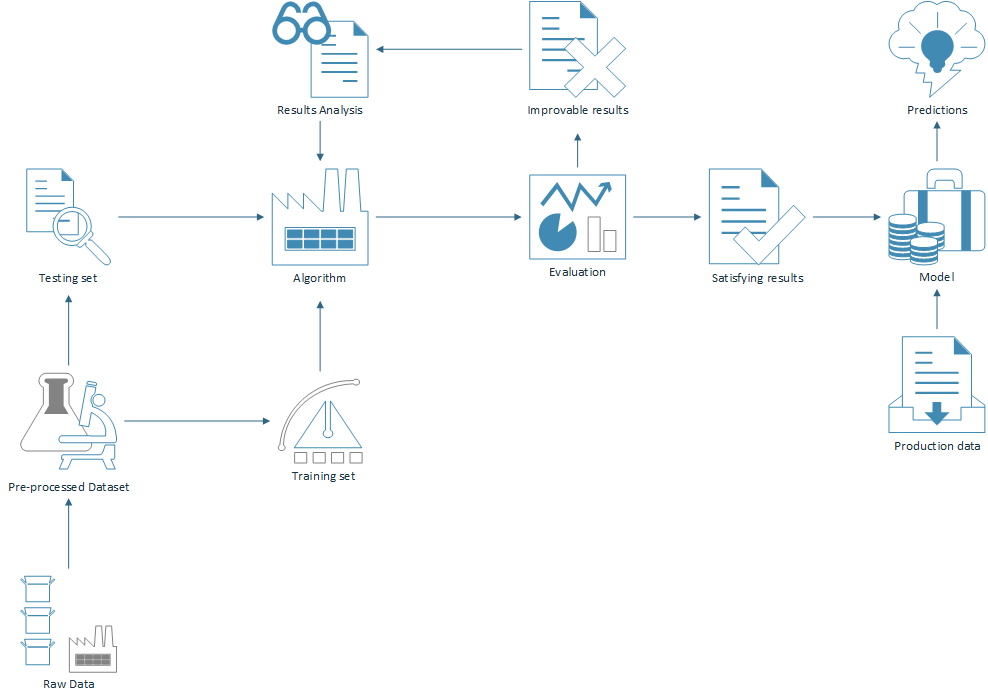
\includegraphics[scale=.55]{img/pers_ml_workflow.png}
The pipeline we created follows the machine learning workflow of a supervised classification problem. We started by curating the dataset, transforming the captures into bro logs. From the bro logs we extracted the list of features and computed all the features. The next processing is the labeling, we used the information related to the malicious hosts and used it to label each one of the features sets. At this point, we have data that can be ingested by supervised algorithms. Before starting to train our models, we do a first analysis of the features and go through the feature selection process. We do a visual analysis of the distributions of the features and a correlation analysis. \\
During this feature selection we create a couple of different sets of features that will will use to train and compare our selections.
We follow by balancing our dataset and we split it into 2 sets, the training set and the testing set. 
We train the classifiers with the different algorithms using the training set. During this training process, we use a feedback loop to change the features used and test out different hyper-parameter optimization techniques. We then test the predictions of our classifiers against the testing set. And finally, we analyze our results and draw some conclusions on our experiment.
\section{Environment}
To build our experiment we used, Python 2 as our programming language. This choice was done because the machine learning libraries available for this programming language are very extensive and they have been adopted largely by the data science community. The libraries related to data science that were used in the project are the following: pandas, numpy, scikit-learn, bro, pcap.\\
All the machine learning algorithms used were part of the scikit-learn library except for XGBoost which was installed with separately.
\\
Some of the features needed some very specific data. To compute the n-grams \cite{ngrams} features we used a repository called the Natural Language Corpus Data that provided all the necessary stats around the most common used n-grams in the internet for legitimate sites.
\\
All the datasets were extracted with a 16 Gb or RAM laptop with an i5 8th Gen processor. All features were computed with the same laptop.
\section{Datasets}
This is a crucial part of the research, based of the approach datasets will be different and the dataset used will influence all the results obtained and will be a big part of the discussions.
\\
For supervised approaches, there is a need of labeled data. We have searched for DNS traffic coming from Botnets combined with Normal traffic. This is a very difficult task because there aren't many datasets that focus on DNS data generated by botnets. It is also difficult because those datasets are complicated to produce and they would take a lot of time if they had to be labeled manually.
\\
The datasets used in this thesis come from different sources that try to provide labeled data or precise data from botnets. These different sources are the CIS (Canadian institute of Security) that provide datasets created for the research related to security on traffic, specifically for machine learning techniques. They have labeled data from a lot of different sources and protocols. The one they provided me focused on different types of botnets.\\
The ISOT Botnet dataset \cite{isot} which consists in a large dataset regrouping 9 malicious botnets traffic in a controlled environment. \\
And finally, the Czech Technical University (CTU) scenarios. They created a project called the Malware Capture Facility (MCFP) to provide researchers with botnet captures. Their repository holds currently more then 300 captures of botnets.
\\
Now that we had the labeled malicious traffic we needed normal traffic to use for our classifiers. We decided to use the traffic provided by CTU. 
\section{Purpose of datasets}
The idea of having different datasets allows to test out our classifiers against completely new data. If some techniques work against a large variety of evasion techniques or on specific ones. It is a way to propose a more robust set of features for complete detections.
\\
Finding proper datasets with botnet traffic with malicious DNS traces is not an easy thing to achieve. Luckily, the CIC team were kind enough to allow me to use their dataset designed for botnet traffic analysis. We also found a dataset proposed by the CTU which is a set of 13 scenarios that represent different types of malicious traffic generated by botnets. The CTU dataset was not as rich in DNS traffic as the other ones, but provided with fast flux traffic to test some of the features proposed to detect FF.

\subsection{CTU}
%\subsubsection{Sources}
%	Already mentioned
%\subsubsection{Content}
%	What are the botnets analyzed
%\subsubsection{Labeling}
%	How did we label them?
%\subsubsection{Use}
%	How did we use it in the study, we tested for example datasets for full training and testing, maybe we used certain datasets to train and others to test. Give more detail
This is a set of datasets provided by the malware capture facility project\cite{CTU}. It captures malicious traffic from different malwares then provide them to the public for research. They also provide their own analysis on most of the datasets which provides insight on how the malware act and how it can be detected.\\
Their main project is called MCFP-13 which is a dataset of 13 scenarios using botnet traffic analyzed and labeled. Their captures provide a lot of different formats which is very helpful when trying to use different datasets and group them together. They also provide hundreds of additional datasets but that are not as well documents and presented which makes their research more complicated.

\subsection{CIC}
%\subsubsection{Source}
%	Already mentioned
%\subsubsection{Content}
%	What are the botnets analyzed
%\subsubsection{Labeling}
%	How did we label them?
%\subsubsection{Use}
%	How did we use it in the study, we tested for example datasets for full training and testing, maybe we used certain datasets to train and others to test. Give more detail
This is a dataset maintained by the Canadian Institute for Cybersecurity\cite{cic} (CIC). The have compiled malicious traffic from different sources and for most of them the traces are labeled which is very convenient for machine learning supervised approaches.\\ 
The dataset they provide for Botnet traffic analysis is composed of 9 different Botnets and of 2 datasets, a training and a testing dataset. Unfortunately, even being the largest labeled  dataset, the DNS traffic was a very low proportion of the malicious traffic. 

\subsection{ISOT}
%\subsubsection{Sources}
%	Already mentioned
%\subsubsection{Content}
%	What are the botnets analyzed
%\subsubsection{Labeling}
%	How did we label them?
%\subsubsection{Use}
%	How did we use it in the study, we tested for example datasets for full training and testing, maybe we used certain datasets to train and others to test. Give more detail
This is a dataset specifically build around DNS traffic by the The ISOT Lab from the University of Victoria. It regroups 9 exploit kits ran in virtual environments in a closed network with a custom DNS server to sniff all the traffic. This dataset provides us with 3 sets of traces, malicious, benign and a mixed\cite{isot}.
	
\section{Dataset Processing}
Because of the amount of different features tested in the thesis. I decided to use 2 pcap extractors. The first was provided by our teacher Prof. J. Colin which is a very effective extractor and summarizes very well the relevant data for most of the features but for labeling and some of the features, more information was required. What we did to obtain a second extractor to complement the information was to run the traffic datasets through Bro, the network IDS. This provided us with DNS.logs, that we then converted using the python "bat" library which converts directly bro logs to dataframes.\\
Most of the labeled datasets actually only provided the IP addresses of the malicious traffic, this is why working with the bro logs was essential to label the datasets.
\subsection{cleaning}
For the cleaning of the dataset we checked for any data that was corrupted or missing, luckily the datasets used didn't have any of these problems. 
\subsection{Scaling}
To solve the problems of scaling introduced when analyzing multiple features we decided to use a panel of techniques and assess which one of them would perform better. \\
We know that normalization and standardization are the main techniques used to solve this issue but this article \cite{normstd} proposed to actually test other techniques because depending on the data they might provide better results. \\
The techniques we tested are the following: StandardScaler (standardization), MinMaxScaler(normalization), RobustScaler, QuantileTransformer (uniform and normal distributions), PowerTransformer and Normalizer.
\subsection{balancing the datasets}
It is very important in supervised learning to balance the dataset or the majority class would mistrain the classifier and output biased results. You could obtain really good accuracy scores but then fail totally at predicting any new data, because you would actually simply predict the majority class. To balance the dataset we decided to down-sample the data from the majority class in a 50:50 ratio.\\

\subsection{Assessment model (for features and models)}
To improve our results we did the following, we used a first loop scaling the data in one of the 7 techniques. We initiated the different algorithms we wanted to test in the second loop, each one of them assigned a parameter grid for the hyper-parameter optimization. Finally, we created different subsets of data with different features to test out the best combinations and our feature selection choices.\\
We then used the metrics explained in chapter 5 (results) to assess the different parameters, options and sets used.

\section{Machine algorithms}
\subsection{Algorithm selection}
Based on popular algorithms used to solve this type of problems and popular algorithms used for classification we decided to test the following algorithms to create the best classifier.
\subsubsection{Gaussian Naive Bayes}
This comes from the know probability and statistics Bayes' theorem. "It describes the probability of an event , based on prior knowledge of conditions that might be related to the event"\cite{bayes}. In ML learning the model saves the probabilities of each feature to belong to which category and when it is asked to predict new data, it does so by computing the event's probability to belong to each one of the categories. It bases its predictions on previous experience.

\subsubsection{K-Nearest Neighbors}
k-Nearest Neighbors (kNN) is a very simple supervised ML algorithm. kNN classifies new objects based on their nearest neighbors. The parameter k represents the amount of nearest neighbors it looks for before it assigns the majority. The model created by kNN is actually the entire training dataset since it will use all the neighbors to determine the classification of a new item. kNN algorithm works well with a low amount of features, with datasets with large dimensions computing the distances for the k-nearest neighbors becomes computationally expensive.

\subsubsection{Decision Trees}
Decision Trees(DTs) are supervised algorithms that based on observations of labeled data creates a model of decision that is represented by a tree where all the nodes of the tree are a condition for the features and where all the leaves are the label they are classified as. The classification process starts at the root and ends in one of the leaves.\\
DTs are very simple to visualize and perform really well even in higher dimensions. The most common problem of DTs is the overfitting of the data. Because outliers and unbalanced datasets will create branches that don't generalize the data correctly.

\subsubsection{Logistic Regression}
Logistic regression (LR) is a simple algorithm that is very effective in binary classification. Its core is the logistic function which transforms ranges of real-values into [0-1] ranges. What the logistic regression algorithm will do is through the use of weights of features, create the logistic function (model) for 1 of the classes and then for new values, it will output a probability which can be seen as a prediction of the input belonging to the class or not \cite{lr}.

\subsubsection{Support Vector Machine}
Support Vector Machine (SVM) is a supervised algorithm that excels in classification problems. The algorithm looks locally between the classes what hyper-plane separates them. 
Its hyper parameters are very interesting too, they allows to adapt to the dimension of the features to allow for transformations of the hyper-planes relative to the dimension. They also allow to tune how much we accept outliers. The tuning has to be done with care because we could end in an overfitting situation that doesn't generalizes enough and therefore could perform poorly with new data.

\subsubsection{XGBoost and Adaboost}
Both algorithms, eXtreme Gradient Boosting (XGBoost) and Adaptive Boosting (AdaBoost), are based on a similar concept which is boosting. Boosting is a technique that modifies weak learners into strong learners. It is done by training multiple of these weak learners sequentially and each improving based on the previous one.\cite{boosting} Both use this technique with different approaches to it.

\paragraph{AdaBoost}
The boosting used with Adaptive Boosting(AdaBoost) is simpler than XGBoost, it uses decision trees with a single decision node, they are called decision stumps. Each mistake made by stumps during classification are forwarded to the next stump by carrying more weight. This will allow the errors to be corrected of the numbers of stumps and obtain a cleaned up result in the end. This concept is mostly applied with DTs but it could be applied to any supervised algorithms. As are trees, AdaBoost are victims of outliers but they do a good job not to overfit the models as its peer. 

\paragraph{XGBoost}
The type of boosting used with XGBoost \cite{xgboost} is Gradient Boosting on steroids. The algorithm improved is the RFs which is already a really strong supervised classifier. Like the AdaBoost, it sequentially improves the current tree using its predecessor but instead of adding more weight to the misclassified observations, it tries to train the next predictor to those observations. But this isn't all, XGBoost was created for fast and high performance to solve the slow characteristic of gradient boosting. That is where the eXtreme part comes in and where they introduced solutions to its shortcomings: parallelization of the tree construction,  distributed computing, out-of-core computing and cache optimization. Due to this, it is one of the most popular algorithms because it provides the best performance on a range of difficult machine learning tasks. Its only drawback is its overfitting but that can be solved fine-tuning its hyper-parameters and its results' interpretation which can be complicated.

\subsubsection{Random forest}
The Random Forest (RF) algorithm is an improvement of the DTs. The concept is to randomly create low correlated models (forest) and give them the same input. It then picks the majority result as the prediction for the input. This technique provides a good way to protect from the overfitting that DTs are known for and to protect against individual errors of the trees. RF takes advantage of Bagging (Bootstrap aggregation) and Feature randomness to achieve this uncorrelated forest.
Bagging consists in giving all the trees the same amount of data but with replaced data (duplicates). Secondly feature randomness as its name implies, at each node the trees only take decision based on a subset of features\cite{rf}.

\subsubsection{Artificial Neural Networks}
Artificial Neural Networks (ANN) is an algorithm created similar to how the brain works and its learning capabilities by modeling neurons and their synapses. It works as a black box system with inputs on one side and and outputs on the other which are dependent on the inputs. The black box is a network of neurons grouped in layers, neurons of each layer connect with the ones of the next layer with weighted connections that will determine when the neurons fire. The modeling is around finding the values of the neurons and the connections inside the black box (hidden layers). The way ANNs hidden layers are computed are through gradient descent, a way of automatically updating the weights step by step into a direction that will make them less wrong, based on the output desired\cite{ann}.

\subsection{Feature selection}
The goal of this step is to avoid using multiple features that provide the same information. This adds more time to the extraction and to the training of the classifiers. As explained in the Machine learning section of the state of the art, there are some common techniques one can use to achieve this: PCA, LDA are really good but introduce difficulties of interpretation of when downsizing features. Univariate feature selection modules from scikit-learn selects the features based on scoring. Manual combination of features and visual analysis can help too understand the features and their relevance.\\
The techniques used will be detailed in the next chapter.

\subsection{Training and testing model}
For the training and testing part of the experiment, we followed the norm and divided the dataset into  a training and testing sets with a 80:20 ratio to provide as much data possible to train the classifier but enough data as well for the testing set to provide substantial statistical value when using it for prediction scores.\\
Furthermore, we used the 10-k fold cross validation technique for the training set to use the best generalization of the data possible \cite{fitting}.\\
We decided to leave KNN and SVM out of the algorithms sets because we realized during the training period that the dimension of features was to high for those algorithms to build models in a reasonable time.